\documentclass{template/openetcs_report}
% Use the option "nocc" if the document is not licensed under Creative Commons
%\documentclass[nocc]{template/openetcs_article}
\usepackage{lipsum,url}
\usepackage{supertabular}
\usepackage{multirow}
\usepackage{color, colortbl}
\definecolor{gray}{rgb}{0.8,0.8,0.8}
\usepackage[modulo]{lineno}
\graphicspath{{./template/}{.}{./images/}}

\begin{document}
\frontmatter
\project{openETCS}

%Please do not change anything above this line
%============================
% The document metadata is defined below

%assign a report number here
\reportnum{OETCS/WP4/D4.3.3V0.0}

%define your workpackage here
\wp{Work-Package 4: ``Validation \& Verification Strategy''}

%set a title here
\title{openETCS Safety case for tool chain and processes}

%set a subtitle here
\subtitle{Process and Toolchain verification for the openETCS on-board unit software development}

%set the date of the report here
\date{November 2015} %\\ Revised April 2015}

%document approval
%define the name and affiliation of the people involved in the documents approbation here
\creatorname{Jan Welte]}
\creatoraffil{TU Braunschweig}

\techassessorname{Abdelnasir Mohamed}
\techassessoraffil{AEbt}

\qualityassessorname{Veronique Gontier}
\qualityassessoraffil{All4Tec}

\approvalname{Klaus-R\"udiger Hase}
\approvalaffil{DB Netz}

%define a list of authors and their affiliation here

\author{Jan Welte}
\affiliation{Technische Universität Braunschweig\\
  Institute for Traffic Safety and Automation Engineering\\
  Hermann-Blenk-Str. 42\\
  38108 Braunschweig, Germany\\
  eMail: openetcs@iva.ing.tu-bs.de \\
  WebSite: www.iva.ing.tu-bs.de}
  
\author{Raphaël Faudou}
\affiliation{Samares Engineering on behalf of ENSEEIHT}

  
%add yourself as author, if you contributed to the document



% define the coverart
\coverart[width=350pt]{openETCS_EUPL}

%define the type of report
\reporttype{Output Document}


\begin{abstract}
This document addresses the general quality and safety assurance concept implemented and applied by the openETCS development process and its supporting toolchain. Thereby, the it is shown how the overall openETCS development process principals presented in D2.3 and  additional document can be applied for a CENELEC confirm SIL 4 development, if the interfaces to the system development are complemented accordingly. For the generic safety argumentation it is shown hw the model design addresses the ETCS system hazards for the OBU Kernel.

\end{abstract}

%=============================
%Do not change the next three lines
\maketitle
\tableofcontents
\listoffiguresandtables
\newpage
%=============================

\chapter{Document Control}

\begin{tabular}{|p{4.4cm}|p{8.7cm}|}
\hline
\multicolumn{2}{|c|}{Document information} \\
\hline
Work Package &  WP4  \\
Deliverable ID & D 4.3.3\\
\hline
Document title & Process and Toolchain verification for the openETCS on-board unit software development \\
Document version & 0.1 \\
Document authors (org.)  & Jan Welte (TU-BS)\\
\hline
\end{tabular}

\begin{tabular}{|p{4.4cm}|p{8.7cm}|}
\hline
\multicolumn{2}{|c|}{Review information} \\
\hline
Last version reviewed & \\
\hline
Main reviewers (org.) & \\
\hline
\end{tabular}

\begin{tabular}{|p{2.2cm}|p{4cm}|p{4cm}|p{2cm}|}
\hline
\multicolumn{4}{|c|}{Approbation} \\
\hline
  &  Name & Role & Date   \\
\hline  
Written by    &  Jan Welte & WP4-T4.4 Task Leader  &  November 2015\\
\hline
Approved by & -- & -- & \\
\hline
\end{tabular}

\begin{tabular}{|p{2.2cm}|p{2cm}|p{3cm}|p{5cm}|}
\hline
\multicolumn{4}{|c|}{Document evolution} \\
\hline
Version &  Date & Author(s) & Justification  \\
\hline
0.1 & 18/10/2013 & Jan Welte &  Document creation \\
\hline  
%0.1 & 28/01/2014 & Jan Welte &  Extended Introduction  \\
\hline  
\end{tabular}
\newpage

% The actual document starts below this line
%=============================

\mainmatter

\chapter{Introduction}
\label{sec:introduction}

 The CENELEC standards EN 50126, EN 50128 and EN 50129 provide a basic life cycle process with specific artifacts which have to be produced during a system development. In this context presents the EN 50128 the specific life cycle and its artifacts for the software development. As this software operates in the system context it has to be defined in the system context which hazards have to be avoided or reduced to reach the required safety level. In this context safety is understood as protecting humans from harm resulting from the system as distinguished from security which covers protecting the system itself from hazards coming from the outside. To  do so the CENELEC standards can only provide guidelines how safety for a system shall be determined and assured by providing certain quality and safety management principles. These have to be adopted to the development methods applied during the system development. 
 
 As the openETCS project is related to a number of different system definitions like the overall railway system, the on-board unit, the kernel software and the development tool chain different safety aspects have to be taken in consideration. Only a small number of these can actually be determined in the openETCS context alone. Respectively, this document and all considerations concerning safety in openETCS are focusing on the principal functional safety of the openETCS on-board kernel software and it resulting principals which have to be applied if the software model and code shall be used in a specific context. To do so the specific development concept of openETCS is set in context to the CENELEC requirements and the underlying quality and safety management principals are shown to be integrated into the overall system management principal during further application of the openETCS results.


\section{Purpose}
\label{sec:purpose}

The hazard and risk analysis activities are part of the overall safety process which is defined in the EN 50129 as "the series of procedures that are followed to enable all safety requirements of a product to be identified and met". To ensure that the safety process is implemented and followed in a proper way during the development the EN 50129 requires a safety management. The management has to present and control all related activities and documentation over the life-cycle taking into account the approval mile-stones and review requirements. As the product life-cycle is an ongoing process and iterative changes are taking place, the management system has to ensure that the respective safety effects of every change is considered. The openETCS project does not cover the full development of an ETCS on-board unit, the tool and process verification in WP 4 and the resulting generic safety case are just providing confirmations how the openETCS toolchain and development process address safety relevant aspects at interface and in kernel design as well as requirements resulting for the use of openETCS kernel outputs. Hence, the purpose of this document is to provide an overview about the underlying quality and safety concepts established at the openETCS development.

As the movement characteristics of a train set specific limits in which a driver alone is able to avoid derailment or any kind of collisions, railway signaling and protection systems have been developed to ensure safe train movements. Respectively, the major parts of a train control system like ETCS includes functionalities which shall guarantee that the overall railway system does not get in a hazardous situation. Correspondingly, this document illustrates where identify hazards from the overall system analysis - if they are related to the openETCS software -  have been addressed in the development process and the kernel design. 

As the openETCS project does not produce an implemented train borne on-board system, the openETCS documents will not cover all specific software and hardware aspects which the EN 50129 requires for a sufficient safety case. Respectively, the openETCS results cannot be used without further work to demonstrate that a derived product using the openETCS kernel is compliant with all specified safety requirements. On this grounds WP 4 has arranged required information for the further use of the openETCS model as a generic safety case.

\section{Document Structure}
\label{sec:document-structure}

Although the openETCS software development process and the respective tool chain are closely connected, certain aspects should by address separately. The chapter \ref{toolchain} first presents the openETCS toolchain concepts and describes the tool classes categorization in the overall context. In addition the resulting qualification needs are addressed. Afterward, presents chapter \ref{sec:development-process} the development process of the openETCS and its artifacts. These are set in relation to the CENELEC lifecycle to address the needed interactions to adopted the openETCS kernel in a specific system development. As traceability is the core cross functionality for quality and safety management and central for reuse of software products and assessment, the final openETCS traceability concepts is presented additionally. The basic results how the existing ETCS system hazards have been addressed during the development is presented in chapter \ref{sec:safetycase}. Thereby, the four main safety case aspects system definition, quality management, safety management and functional safety are addresses separately.

\section{Document Evolution}

This document is based on the results of the various iterations during the WP 4 work and shall present the overall concept for the openETCS development. As the openETCS ETCS OBU reference model is an ongoing development, this document can not provide a final status which can be used as a assessable safety case for the direct implementation. However this document presents the concept and principals applied in openETCS which can be used and extended to integrate the OBU reference model in specific applications.

The openETCS development plan presented in chapter \ref{sec:development-process} is based on the current version of the Quality Assurance Plan, the D2.3 deliverables group discribing the development process and WP 7 outputs concerning the toolchain. Concrete methods to verify and validate safety relevant properties derived from the hazard control methods described in this document, are presented in depth   in the Verification and Validation plan and the specific results are documented in are respective verification and validation reports.

\section{Reference Documents}
\label{sec:refdoc}

This document essentially refers to the following standards, ETCS specification documents and openETCS project documents.

\begin{itemize}
\item \textbf{ISO~9000} --- 12/2005 --- \emph{Quality management}
\item \textbf{ISO~9001} --- 12/2008 --- \emph{Quality management systems — Requirements}
\item \textbf{ISO~25010} --- 03/2011 --- \emph{Systems and software engineering -- Systems and software Quality Requirements and Evaluation (SQuaRE) -- System and software quality models}
\item \textbf{CENELEC EN~50126-1} --- 01/2000 --- \emph{Railways applications –- The specification and 
demonstration of Reliability, Availability, Maintenability and Safety (RAMS) –- Part 1: 
Basic requirements and generic process}
\item \textbf{CENELEC EN~50128} --- 10/2011 --- \emph{Railway applications -- Communication, signalling and 
processing systems -- Software for railway control and protection systems}
\item \textbf{CENELEC EN~50129} --- 05/2003 --- \emph{Railway applications –- Communication, signalling and 
processing systems –- Safety related electronic systems for signalling}
\item \textbf{CCS~TSI} --- \emph{ CCS TSI for HS and CR transeuropean rail has been adopted by a Commission Decision 2012/88/EU on the 25th January 2012}
\item \textbf{SUBSET-026} 3.3.0 --- \emph{System Requirement Specification}
\item \textbf{SUBSET-091} 3.2.0 --- \emph{Safety Requirements for the Technical Interoperability
of ETCS in Levels 1 \& 2}
\item \textbf{SUBSET-088} 2.3.0 --- \emph{ETCS Application Levels 1 \& 2 - Safety Analysis}
\item \textbf{OpenETCS FPP} --- \emph{Project Outline Full Project Proposal Annex OpenETCS} -- v2.2
\item \textbf{OpenETCS D2.2} -- Report on CENELEC standard
\item \textbf{OpenETCS D2.3} -- Definition of the overall process for the formal description of ETCS and the rail system it works in 
\item \textbf{OpenETCS D2.4} -- Definition of the methods used to perform the formal description
\end{itemize}


%%%%%%%%%%%%%%%%%%%%%%%%%%%%%%%%%%%%%%%%%%%%%%%%%%%%%%%%%%%%%%%

\section{Glossary}
\label{sec:glossary}



\begin{tabular}{rl}
\textbf{ACedit} & Assurance Case Editor \\ 
\textbf{ARM} & Argumentation  Metamodel \\ 
\textbf{ETCS} & European Train Control System \\ \textbf{ERA} & European Railway Agency \\ \textbf{FMEA} & Failure Mode Effect Analysis \\ 
\textbf{GSN} & Goal Structured Notation \\ 
\textbf{MoRC} & Management of Radio Communication \\ 
\textbf{RAMS} & Reliability, Availability, Maintainability and Safety \\
\textbf{SIL} & Safety Integrity Level \\ 
\textbf{SRS} & System Requirement Specification \\ 
\textbf{THR} & Tolerable Hazard Rate \\ 
\textbf{V\&V} & Verification \& Validation \\ 
\end{tabular} 




\section{Background Information}
\label{sec:Background}


If specific information are needed the can be place here. (D4.2.3 shall not be repeated)


\chapter{Tool Chain}
\label{toolchain}
\section{Overview}

by Jan Welte

\begin{figure}[h]
\centering
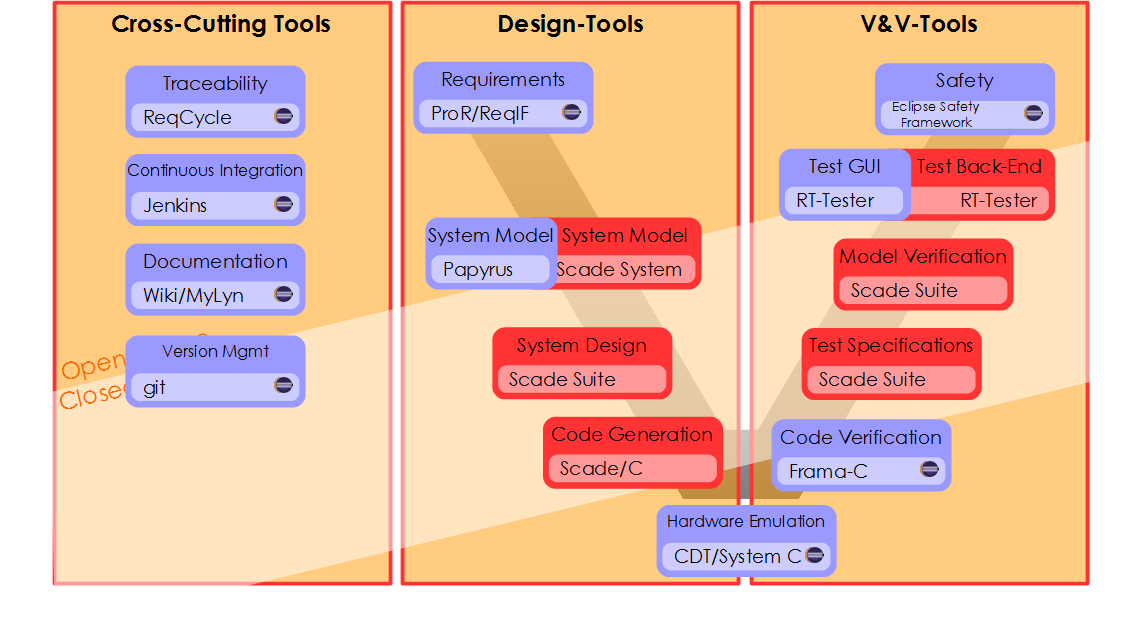
\includegraphics[width=0.9\linewidth]{./images/Toolchain-New-Version-V-Model-Nov-2015}
\caption{Core openETCS Toolchain}
\label{fig:Toolchain-New}
\end{figure}


\section{Tool Qualification}

\begin{center}
\tablecaption{OpenETCS toolchain and categorisation}
\label{tab:ToolCat}
\tablehead{\hline Tool & Support Activity & Tool Class & Justification \\ }
\tabletail{ \hline \multicolumn{4}{|r|}{Continues on next page} \\ \hline}
\tablelasttail{\hline}

\begin{supertabular}[H]{|p{2cm}|p{4cm}|p{4cm}|p{4cm}|}
\hline Papyrus Editor & Definition of the model architecture & T1 & \\
\hline Papyrus SysML checker & Check SysML conformity of the model & T2 & \\
\hline SCADE Editor & Low-level modeling and code generation & T1 & \\
\hline SCADE Code Generator & Code generation & T3 & \\
\hline ProR & Requirements management & T1 & \\
\hline Bitwalker & Generation of data structures for modelling & T3 & \\
\hline Git & Versioning \& Traceability & T1 & \\
\hline RT Tester & Model-based testing & T2 & \\ 
\hline CPN Tools & Model checking and test case generation & T2 & \\
\end{supertabular} 
\end{center}

tool are coming from D7.3 table 1

by Michael Jastram (or other expert from WP7)


broad overview of the toolchain and the status of qualification (generall information can be placed in section Overview)
- which tools have to be qualified
- which tools are qualified? (in which way)
- how should qualification be address for tools with pending qualification

\section{SCADE}

by Jan Welte and Marc Behrens

- use of SCADE for quality assurance
- limitations of SCADE
- addressing safety issues and properties in SCADE 
(potential specific aspects in openETCS deviation from the usual use of SCADE)


\section{Safety Architect}

by FrederiqueVallee (or Francois Revest)

- use of Safety Architect in openETCS (maybe addressing relation to Eclipse Safety Framework)
- function in development process
- inputs and outputs
- results (in general, and specific for openETCS)

\chapter{OpenETCS Development}
\label{sec:development-process}

\section{overview}

by Jan Welte

Short overview of current work.

- Main principals to ensure consistency 

- Mainly collecting findings

- allocate the tools to the process steps used/ qualified

\section{Compatibility to CENELEC standards}

by Mohamed Abdelnasir

- overview results relation to EN 50126/50128 lifecycle 
- reasons for deviations
- additional findings

\section{Traceability}

by @janwelte @raphaelfaudou

- addressing specific position of traceability for safety argumentation
- introducing basic concept
- main findings (limitations)

Requirement traceability activity consists in ensuring that all product engineering artifacts (including verification means) can be traced to an originating stakeholder requirement either directly (direct link) or through other requirements derived from stakeholder requirements. It means creating links but also manage their status (created, confirmed...) and potentially their deletion.

Concerning OpenETCS, there are several needs for traceability but main ones concern definition of links between SRS-Subset 26 requirements and two models:
\begin{itemize}
\item OpenETCS architecture SysML model (System, subsystem, SW functions), edited with SCADE System tool
\item OpenETCS OBU formal executable software model (SW architecture, SW functions, detailed design), edited with SCADE Suite tool
\end{itemize}

Figure \ref{fig:openETCSTraceabilityMainPriority} illustrates all required traceability links needed to achieve current design verification and highlights main priority (arrows with largest size).

\begin{figure}[htbp]
\centering
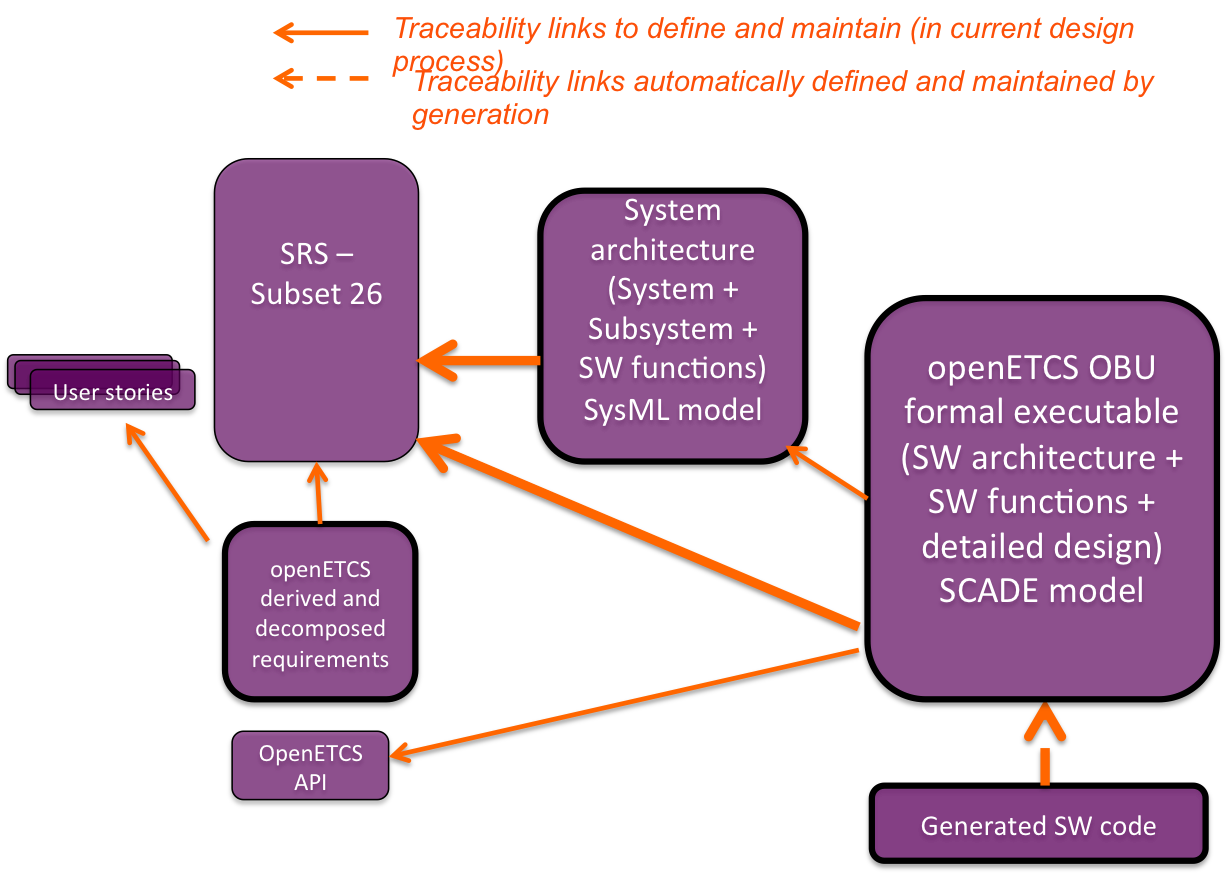
\includegraphics[width=.9\linewidth]
{./images/openETCSTraceabilityMainPriority.png}
\caption{\label{fig:openETCSTraceabilityMainPriority}OpenETCS traceability chains for current design with highlight on main priorities}
\end{figure}

OpenETCS tool chain currently supports ability to create links between:
\begin{itemize}
\item SRS Subset 026 .ReqIF requirements and additional requirements => through ProR integrated tool,
\item SysML architecture model and SRS Subset 026 .ReqIF requirements through ReqCycle integrated tool
\end{itemize}
 
\textbf{Note:} it is also possible to create links between SCADE Model and SRS Subset 026 .ReqIF requirements through SCADE Suite RM Gateway and ReqTify traceability product but it is not an open solution and it requires additional licenses. Therefore that approach was used only by a few partners and was not considered as conclusive. There are pending investigations to provide alternate open solutions to support edition of those traceability links.




\chapter{Generic OpenETCS Safety Case}
\label{sec:hazardandrisk}

\section{System/ Sub-System Definition}

by Jan Welte

- general information concerning openETCs system and sub-system structure
- potential applications for artifacts

\section{Quality Management}

Since the openETCS project as a research does not have the objective to conduct all steps needed for a vital on-board unit development, the resulting safety case will be generic in many parts only giving the requirements and basic safety strategies, but lacking the actual evidence. However, the overall safety argumentation has to be set up to meet SIL 4 requirements. Therefore the safety case has to show that the methods chosen in the openETCS development process satisfy the EN~50128 quality requirements and which documents have to be created during the process to obtain the required evidence. Basis for this work will be the Quality Assurance Plan as this document builds the basis for all quality management activities.

by Mohamed Abdelnasir

- basic concept for quality management in openETCS
- missing aspects in quality management
- main finding to address additional measures to complete quality management

\section{Safety Management}

As detailed in chapter \ref{sec:hazardandrisk} the overall safety argumentation has to demonstrate that during the development process the higher-level safety requirements have been addressed and that accordingly the on-board software satisfies the safety level. The safety case has to specify traces from high-level hazardous events to all subsystem requirements allocated to the openETCS software architecture and their verification and validation. Therefore, the safety case has to present evidence that the chosen methods are sufficient to demonstrate compliance to the requirements and that these methods are applied in a consistent process to ensure that all safety requirements are respected and validated.


by Jan Welte

- basic concept for safety management in openETCS
- missing aspects in safety management
- main finding to address additional measures to complete safety management

\section{Functional/Technical Safety}

Based on the ETCS reference architecture SUBSET-91 defines the role of ETCS as a train protection system the following way:

\begin{center}
\textbf{"To provide the Driver with information to allow  him to drive the train safely and to enforce respect of this information, to the extent advised to ETCS."}
\end{center}

Respectively, the Core Hazard for the ETCS reference architecture is defined as the following in SUBSET-91:
\begin{center}
\textbf{"Exceedance of the safe speed or distance as advised to ETCS."}
\end{center}

Based on the role of ETCS and its respective SIL 4 quantification the maximum allowed rate of occurrence (Tolerable hazard rate) of the ETCS Core Hazard for ETCS on-board is
\[1.0\times10^{-9} hour^{-1} train^{-1}.\]
The same value is specified for the corresponding track-side.

Adapted form the ETCS system safety analysis presented in SUBSET-88 the Annex A of SUBSET-91 presents the List of Hazardous Events inside ETCS that might cause the ETCS Core Hazard to occur, either alone or in combination with other failures. These are the events not eliminated by the operational analysis. 34 of these hazardous events are allocated to the Kernel, which make them the basis for the on-board software hazard and risk analysis. 

\begin{center}
\tablecaption{List of ETCS Kernel Hazardous Events}
\label{tab:KernelHaz}
\tablehead{\hline Event Id. & Event Description & Corresponding performance requirement in Subset-041 & OpenETCS allocation \\ }
\tabletail{ \hline \multicolumn{4}{|r|}{Continues on next page} \\ \hline}
\tablelasttail{\hline}

\begin{supertabular}[H]{|p{2cm}|p{4cm}|p{4cm}|p{4cm}|}
\hline KERNEL-1 & Balise linking consistency checking failure & In case the message is received but the linking is not consistent:
5.2.1.1: Delay between receiving of a balise message and applying the emergency brake
KERNEL-2 &  \\ 
\hline KERNEL-2 & Balise group message consistency check-ing failure  & 5.2.1.1: Delay between receiving of a balise message and applying the emergency brake &  \\ 
\hline KERNEL-3 & Failure of radio message correctness check &  &  \\ 
\hline KERNEL-4 & Radio sequencing checking failure &  &  \\ 
\hline KERNEL-5 & Radio link supervision function failure &  &  \\ 
\hline KERNEL-6 & Manage communication session failure &  &  \\ 
\hline KERNEL-7 & Incorrect LRBG &  &  \\ 
\hline KERNEL-8 & Emergency Message Acknowledgement Failure &  &  \\ 
\hline KERNEL-9 & Speed calculation underestimates train speed & 5.3.1.2: Accuracy of speed known on-board, in ceiling speed monitoring, release speed monitoring and in target speed monitoring in case the compen-sation of the speed measurement in-accuracy is inhibited  &  \\ 
\hline KERNEL-10 & Functional failure of standstill detection &  &  \\ 
\hline KERNEL-11 & Incorrect traction/braking model (e.g. brake use restrictions) &  &  \\ 
\hline KERNEL-12 & Failure of standstill supervision &  &  \\ 
\hline KERNEL-13 & Failure of backward distance monitoring &  &  \\ 
\hline KERNEL-14 & Failure of reverse movement protection &  &  \\ 
\hline KERNEL-15 & Incorrect cab status (TIU failure) &  &  \\ 
\hline KERNEL-16 & Incorrect train status TIU sleeping/cab status &  &  \\ 
\hline KERNEL-17 & Wrong Acceptance of MA &  &  \\ 
\hline KERNEL-18 & Failure to manage RBC/RBC &  &  \\ 
\hline KERNEL-19 & Failure of train trip supervision in OS, LS and FS & 
5.2.1.1: Delay between receiving of a balise message and applying the emergency brake
5.2.1.13: Delay between passing an EOA/LOA and applying the emergen-cy brake  &  \\
\hline KERNEL-20 & Failure of train trip supervision, shunting and SR & 
5.2.1.1: Delay between receiving of a balise message and applying the emergency brake &  \\ 
\hline KERNEL-21 & Incorrect supervision of stop in SR & 
5.2.1.1: Delay between receiving of a balise message and applying the emergency brake &  \\ 
\hline KERNEL-22 & Incorrect current EoA & 
5.2.1.6: Delay between receiving of an emergency message and applying the reaction on-board &  \\ 
\hline KERNEL-23 & Incorrect train position / train data sent from on-board to trackside & 
5.3.1.3: Age of position measurement for position report to trackside
5.3.2.1: Safe clock drift &  \\ 
\hline KERNEL-24 & Failure of message acknowledgement &  &  \\ 
\hline KERNEL-25 & Incorrect traction/braking model (Accelera-tion only) &  &  \\ 
\hline KERNEL-26 & Deleted &  &  \\ 
\hline KERNEL-27 & Incorrect System Data (e.g. current level) &  &  \\ 
\hline KERNEL-28 & Incorrect confidence interval &  &  \\ 
\hline KERNEL-29 & Failure to shorten MA &  &  \\ 
\hline KERNEL-30 & Incorrect shortening of MA &  &  \\ 
\hline KERNEL-31 & Deleted &  &  \\ 
\hline KERNEL 32 & Failure of loop message consistency check-ing &  &  \\ 
\hline KERNEL-33 & Wrong processing of MA information  & 5.2.1.3: Delay between receiving of a balise message and reporting the re-sulting change of status on-board
(5.2.1.4: Delay between receiving of a MA via radio and the update of EOA on-board).
Note: Whether 5.2.1.4 is safety related must be evaluated in the specific ap-plication’s hazard analysis, see further section 5.3.  &  \\
\hline KERNEL-34 & Incorrect supervision of MA time-outs (sec-tions and overlaps) & 
5.2.1.3: Delay between receiving of a balise message and reporting the re-sulting change of status on-board
(5.2.1.4: Delay between receiving of a MA via radio and the update of EOA on-board).
Note: Whether 5.2.1.4 is safety related must be evaluated in the specific ap-plication’s hazard analysis, see further section 5.3.  &  \\
\hline 
\end{supertabular} 
\end{center}

The main evidence for this part will be provided during verification steps, tracing identified hazards and risk control measures and in case where it is possible also validation results showing that the system is not behaving in an unsafe way. Mainly, it shall be demonstrated that all required risk control measures are taken into account in the actual model and/or code. Thereby, it has to be stated which artifacts have to be provided by which role during the development process and which content can be reused for overall safety argumentation in an implementation.

by Jan Welte

- addressing general system safety properties and allocation to functional structure
- listing needed integration properties for "safe" use of software model (specifically interface assumptions)

by Francois Revest

- addressing concrete findings from safety propagation analysis
- additional measures applicable to tackle open points


\chapter{Conclusion}
\label{sec:conclusion}

This document presents the basic concept for the main safety related activities in the openETCS development as they have been determined during the first verification and validation iteration level of WP 4. As these have been done in respect to a still evolving development methodology and tool chain, the overall process as to be detailed and adopted as the project continues. 

In general the verification and validation activities have to ensure that the safety principal apportioned to the on-board functionality are satisfied. Hence, the main objective for the openETCS safety case as presented in chapter \ref{sec:safetycase} is to provide the fundamental quality and safety principles for the openETCS development as these have to be completed by adopters of the openETCS results for their assessment. Therefore, the general safety argumentation and the concrete evidence shall be clear distinguished to ease applicability and support discussions with different legal authorities.

Overall the main methodology for the hazard and risk analysis as well as the safety case work has been defined during the first level iteration but these concepts have to be further refined over the next iterations with the evolving development process.

\bibliographystyle{unsrt}
\bibliography{./ref/ref-HaRA}


%===================================================
%Do NOT change anything below this line

\end{document}


